\subsection{Identity-Transformation Algorithms}
\label{subsec:overview}

We propose the identity transformations on an elliptic curve $\mathbb{E}$,
and Table \ref{tbl:notations-protocol} lists the notations.
Besides, it is easy to shift these transformations into a finite field $\mathbb{F}_q$.
%The subscript $j$ and/or superscript $i$ may be omitted if there is no ambiguity.


\begin{table}[tb]
\footnotesize
    \caption{Notations used in the UPPRESSO protocol}
    \centering
%    \begin{tabular}{|c|c|c|}
    \begin{tabular}{|r|p{6.79cm}|} \hline
    {\textbf{Notation}} & {\textbf{Description}} \\ \hline
    {$\mathbb{E}$, $G$, $n$} & {$\mathbb{E}$ is an elliptic curve over a finite field $\mathbb{F}_q$. $G$ is a base point (or generator) on $\mathbb{E}$, and the order of $G$ is a prime number $n$.} \\ \hline
    {$ID_{U_i}$} & {$ID_U = u \in \mathbb{Z}_n$ is the $i$-th user's unique identity at the IdP, which is known only to the IdP.} \\ \hline
   {$ID_{RP_j}$} & {$ID_{RP} = [r]G$ is the $j$-th RP's unique identity, which is publicly known; $r \in \mathbb{Z}_n$ is known to \emph{nobody}.} \\ \hline
    {$t$} & {$t \in \mathbb{Z}_n$ is a user-selected random integer in each login; $t$ is shared with the target RP and kept unknown to the IdP.} \\ \hline
    {$PID_{RP_j}^l$} & {$PID_{RP} = [t]{ID_{RP}} = [tr]G$ is the $j$-th RP's pseudo-identity, in the user's $l$-th login visiting this RP.} \\ \hline
    {$PID_{U_i,j}^l$} & {$PID_U = [{ID_U}]{PID_{RP}} = [utr]G$ is the $i$-th user's pseudo-identity, in the user's $l$-th login visiting the $j$-th RP.} \\ \hline
     {$Acct_{i,j}$} & {$Acct = [t^{-1}\bmod n]PID_{U} = [ID_U]ID_{RP} = [ur]G$ is the $i$-th user's locally-unique account at the $j$-th RP, publicly known.} \\ \hline
    {$SK$, $PK$} & {The IdP's private key and public key, used to sign and verify identity tokens and RP certificates.} \\ \hline
    {$Enpt_{RP_j}$} & {The $j$-th RP's endpoint for receiving the identity tokens \cite{rfc6749}.} \\ \hline
    {$Cert_{RP_j}$} & {The RP certificate binding $Enpt_{RP_j}$ and $ID_{RP_j}$, signed by the IdP.} \\ \hline
    \end{tabular}
    \label{tbl:notations-protocol}
\end{table}

\noindent {\bf $\boldsymbol{ID_{\boldsymbol{U}}}$, $\boldsymbol{ID_{\boldsymbol{RP}}}$ and $\boldsymbol{Acct}$.}
The IdP assigns a unique random integer $u \in \mathbb{Z}_n$ to a user (i.e., $ID_U = u$),
 and randomly selects unique $ID_{RP} = [r]G$ for an RP. % if it is a point on $\mathbb{E}$.
Here, $G$ is a base point on $\mathbb{E}$ of order $n$, and $[r]G$ denotes the addition of $G$ on the curve $r$ times.
$Acct_{i,j} = \mathcal{F}_{Acct\ast}(ID_{U_i}, ID_{RP_j})= [ID_{U_i}]ID_{RP_j} =[u_ir_j]G$ is automatically assigned to a user at every RP.

A user's accounts at different RPs are inherently different and unlinkable.
A user's identity $ID_U = u$ is unknown to all entities except the honest IdP; otherwise, colluding RPs could calculate $[u]ID_{RP_j}$ for any known $u$ and link these accounts.
Meanwhile, $ID_{RP} = [r]G$ and $Acct = [ID_U]ID_{RP}$ are publicly-known,
 but $r$ is always kept secret;
otherwise, two colluding RPs with $ID_{RP_j} = [r]G$ and $ID_{RP_{j'}} = [r']G$ could link a user's accounts by checking whether $[r']Acct_j$ is equal to $[r]Acct_{j'}$ or not.

Fortunately, in UPPRESSO $r$ is processed only once by the IdP,
    while $u$ is used only by the IdP internally and
 not enclosed in any message; see Section \ref{implementations} for details.


\noindent {\bf $\boldsymbol{ID_{\boldsymbol{RP}}}$-$\boldsymbol{PID_{\boldsymbol{RP}}}$ Transformation.} When visiting an RP,
a user selects a random number $t \in \mathbb{Z}_n$
    and calculates $PID_{RP}$ as below. She also sends $t$ to the RP.
\begin{equation}
PID_{RP} = \mathcal{F}_{PID_{RP}}(ID_{RP},t) = [t]{ID_{RP}}
\label{equ:PIDRP}
\end{equation}

% = [tr]G

%In each login, the user selects $t$ and shares it with the RP to negotiate $PID_{RP}$. 
%--removed due to double-check discussion
%It makes no difference if the RP selects $t$ randomly and sends it to the user, as long as both of them calculate $PID_{RP}$ \emph{independently} and check if the received $PID_{RP}$ is equal to the calculated one.

\noindent {\bf $\boldsymbol{ID_U}$-$\boldsymbol{PID_U}$ Transformation.}
On receiving an identity-token request for $PID_{RP}$ from a user authenticated as $ID_U$, the IdP calculates $PID_{U}$ as below.
\begin{equation}
PID_{U} = \mathcal{F}_{PID_U}(ID_U, PID_{RP}) =
  [{ID_U}]{PID_{RP}}
 \label{equ:PIDU}
\end{equation}

% = [utr]G

\noindent {\bf $\boldsymbol{PID_U}$-$\boldsymbol{Acct}$ Transformation.}
%The user sends $t$ to the target RP as a trapdoor to derive her account.
After verifying a signed identity token, the RP calculates $Acct$ as follows.
\begin{equation}
Acct = \mathcal{F}_{Acct}(PID_{U},t)
   = [t^{-1} \bmod n]PID_{U}
   \label{equ:Account}
\end{equation}

The above identity transformations ensure \emph{account uniqueness}:
    At an RP, every user owns a unique account, because $ID_{RP} = [r]G$ is also a generator of $\mathbb{E}$ and then
     $Acct = \mathcal{F}_{Acct\ast}()=[ur]G$ is unique at this RP.

Meanwhile, in a login involving no adversary,
 the visited RP always derives the account belonging to the user who requests the identity token,
    by calculating $\mathcal{F}_{Acct}(PID_{U}, PID_{RP})$.
%\emph{Account correctness} is satisfied:
%The visited RP derives an identical account for a user in her different logins,
%    which is exactly the user's permanent account at this RP.
From Equations \ref{equ:PIDRP}, \ref{equ:PIDU}, and \ref{equ:Account}, it is derived that
\begin{equation}
   Acct =  [t^{-1}utr]G = [ur]G = \mathcal{F}_{Acct\ast}(ID_U, ID_{RP})
   \label{equ:AccountNotChanged}
\end{equation}


In Section \ref{sec:analysis},
    under the adversarial scenarios, we formally prove the other required properties (i.e.,
    user identification, RP designation, IdP untraceability, and RP unlinkability) of the identity transformations.
% Note that the proofs in Section \ref{sec:analysis} consider adversaries.

\subsection{The Designs Specific for Web Applications}
\label{sec:web-design}

When the required properties of identity transformations are satisfied,
    in UPPRESSO we need to additionally ensure:
\begin{itemize}
  \item Authenticity, confidentiality, and integrity of identity tokens,
  by the common mechanisms in widely-deployed SSO services \cite{OpenIDConnect, rfc6749, SAML,GoogleIdIntegrate,de2014oauth,FettKS14,BrowserID,uber},
  \item $PID_{RP} = [t]{ID_{RP}}$ is calculated based on the target RP's identity but not any other RPs' (i.e., the target RP is designated) and $t$ is known only to the target RP and the initiating user (but not the honest IdP; otherwise, the IdP is able to calculate $ID_{RP}$ by itself),
  \item 
No direct privacy leakage in the requesting, receiving and forwarding of identity tokens
(e.g., no HTTP \texttt{referer} header about the RP server is leaked to the IdP in HTTP requests).
\end{itemize}

In an original OIDC system with pop-up UX, as shown in Figure \ref{fig:OpenID},
%there is a user-i window responsible for communicate with the IdP (i.e., request an identity token after user authentication and attribute authorization) and a user-r window to communicate with the visited RP (i.e., receive the token). In particular,
    a user requests a token by sending the target RP's identity (i.e., $ID_{RP}$) via the user-i window,
%For instance, in OIDC services with redirect UX, an RP's endpoint to receive tokens is stored as the \texttt{redirect\_uri} parameter at the IdP.
%The IdP employs HTTP 302 redirection to send tokens to the RP, by setting this parameter as the target URL in the HTTP response to a user's identity-token request \cite{OpenIDConnect}.
%  % so the user agent (i.e., browser) forwards it to the designated RP.
%Alternatively, 
    and the IdP replies with the signed token and also the RP's endpoint to receive tokens (i.e., $Enpt_{RP}$).
Then, after receiving the token, the user-i script forwards it to the user-r script by \verb+postMessage+
    which is restricted by the origin of $Enpt_{RP}$ \cite{SPRESSO,MITREid,BrowserID,GoogleIdIntegrate,de2014oauth,OpenIDConnect}.
The \verb+postMessage+ targetOrigin mechanism \cite{postm-targeto} restricts the recipient,
so this ensures confidentiality of identity tokens because (\emph{a}) only scripts downloaded from the origin of $Enpt_{RP}$ are legitimate recipients of the forwarded tokens
    and (\emph{b}) the relationship between $Enpt_{RP}$ and $ID_{RP}$ is maintained at the honest IdP server.

%The following designs are proposed, %\footnote{UPPRESSO also works with redirect UX, .}
%    and the complete UPPRESSO protocol is described in Section \ref{implementations}.
In UPPRESSO the IdP receives $PID_{RP}$ (but not $ID_{RP}$),
    so it cannot reply with $Enpt_{RP}$ to the user-i window.
%
%The user's operations, e.g., request redirection, authorization, and token forwarding, are performed by user agents, such as a browser for web applications.
%
Thus, in each login, 
as shown in Figure \ref{fig:process},
when the user-i window is popped up,
    the RP certificate (i.e., $Cert_{RP}$) and the scope of request user attributes are also carried with the HTTP request to the IdP,
    which is generated by the user-r script.
This HTTP request downloads the user-i script,
    which in turn verifies $Cert_{RP}$ to extract $ID_{RP}$ and $Enpt_{RP}$, and calculates $PID_{RP} = [t]ID_{RP}$. % that binds $ID_{RP}$ and $Enpt_{RP}$.
Then, after the IdP signs the token,
    the user-i script forwards it to the user-r script by \verb+postMessage+,
    which is also restricted by the origin of $Enpt_{RP}$.
This ensures that (\emph{a}) $PID_{RP} = [t]{ID_{RP}}$ is calculated based on the visited RP's identity and (\emph{b}) the identity token is forwarded to the corresponding RP server,
    because $Enpt_{RP}$ and $ID_{RP}$ are signed in $Cert_{RP}$ by the IdP.

In the HTTP request to pop up the user-i window, $Cert_{RP}$ and the scope of requested user attributes are carried as \emph{fragments} (but not parameters) \cite{url-fragment}, which are identified by \texttt{\#} instead of \texttt{?},
    so that they are not sent to the IdP web server but processed by the browser.
We save $Enpt_{RP}$ and $t$ using the \verb+sessionStorage+ HTML object \cite{sessionStorageHtml},
    because the user-i window is refreshed to finish user authentication and attribute authorization.
%The scripts are responsible for communicating with the origin web servers and also the cross-origin communications within the browser.
% as most browsers do in secure OIDC settings \cite{de2014oauth,GoogleIdIntegrate}.
%\footnote{The user-i script is recommended in OIDC services for an in-context user experience of attribute authorization \cite{GoogleIdIntegrate,uber}, so the authorization of user attributes is also implemented through this user-i script in UPPRESSO.}
Therefore, $Cert_{RP}$, $Enpt_{RP}$ and $t$ are processed locally within browsers.


On receiving an identity-token request, the IdP web server checks the included HTTP \texttt{origin} header to ensure it is sent by the user-i script,
which verifies $Cert_{RP}$ to ensure the correct relationship between $Enpt_{RP}$ and $ID_{RP}$.
The IdP's public key is set in the user-i script to verify $Cert_{RP}$,
so a user configures nothing locally,
 like in other popular SSO systems \cite{OpenIDConnect, rfc6749, SAML, SAMLIdentifier}.
%This should be conducted by an \emph{honest} script that obtains $ID_{RP}$ correctly
%    and does not leak $t$, from which it could calculate $ID_{RP} = [t^{-1}\bmod n]PID_{RP}$.
 %otherwise, it could directly leak the RP's domain to the IdP.\footnote{To eliminate this assumption, we can implement the user-agent functions with trusted browser extensions, which are installed before a user visits RPs.}


%After receiving an identity token from the IdP, the user-i script needs to ensure the user-r script will forward the token to $Enpt_{RP}$ %, which is bound with $ID_{RP}$
%specified in the verified RP certificate.
%As the communications between scripts occurs within COTS browsers using \verb+postMessage+, %To avoid the honest user sending the identity token to an adversary,
%the \verb+postMessage+ targetOrigin mechanism \cite{postm-targeto} restricts the recipient. %(i.e., the RP script).
%When the user-i script sends messages, the recipient's origin is set as a parameter, e.g., \verb+postMessage(tk, 'https://RP.com')+, including the protocol (i.e., \verb+https+), the domain (i.e., \verb+RP.com+), and a port if applicable.
%Only the script downloaded from this targetOrigin is a legitimate recipient.
%This design is commonly used to correctly forward tokens in popular OIDC systems \cite{SPRESSO,MITREid,BrowserID,de2014oauth,OpenIDConnect}.
%
%The \emph{RP certificates} deals with the problem of mapping an identity proof with its targeting RP.
%That is, the IdP script derives the RP's $ID_{RP}$ and origin from the RP certificate, while the $PID_{RP}$ is generated with this $ID_{RP}$. Thus, the IdP script always knows the targeting RP of identity proof, therefore, the \verb+postMessage+ mechanism can guarantee that the identity proof would not be sent to the adversary.

Compared with the original OIDC protocol in Figure \ref{fig:OpenID},
UPPRESSO adopts the common mechanisms for secure communications,
except that the relationship between $ID_{RP}$ and $Enpt_{RP}$ is maintained as $Cert_{RP}$ (i.e., in an offline way by the IdP).
Thus, authenticity, confidentiality, and integrity of identity tokens are still ensured in UPPRESSO.
Meanwhile, we implement the IdP's token endpoint in an OIDC-compatible way \cite{rfc6749,OpenIDConnect}:
        When receiving a token request for an ``unregistered'' $ID_{RP}$ (i.e., $PID_{RP}$),
the IdP issues a token but replies with an ``empty'' $Enpt_{RP}$,
    and the calculation of $PID_{U}$ is considered as a special way to assign PPIDs.
%The IdP's other endpoints (e.g., authorization endpoint, logout endpoint and RP registration endpoint) are kept unchanged.

Finally, to prevent referer leakage in the HTTP request to pop up the user-i window,
 we need to ensure this request does not carry an HTTP \texttt{referer} header, which reveals the visited RP's domain to the IdP web server.\footnote{In original OIDC services similar privacy leakages commonly exist, but do not matter because such services are not designed to prevent IdP-based login tracing.} %Generally, when a browser window visits another website not belonging to its opener's origin, the HTTP request to this website automatically carries a \texttt{referer} header (i.e., the opener's origin). Such an HTTP header leaks the visited RP's domain to the IdP.
%
%Fortunately, in UPPRESSO this pop-up is an HTTP redirection from the new window to the IdP (Steps 1.2-1.3 in Figure \ref{fig:process}), but not a direct visit. The HTTP redirection response from the RP server includes a \texttt{referrer-policy=no-referrer} header, which ensures that the HTTP request to access the IdP carries no \texttt{referer} header.
This is achieved by setting
\verb+<meta name="referrer" content="no-referrer">+
in the RP's SSO login page \cite{referer_policy}.
%This method is specified by W3C \cite{referer_policy} and widely supported. We have tested it in various browsers such as Chrome, Safari, Edge, Opera, and Firefox, and confirmed no referer leakage.

\begin{figure*}[htb]
  \centering
  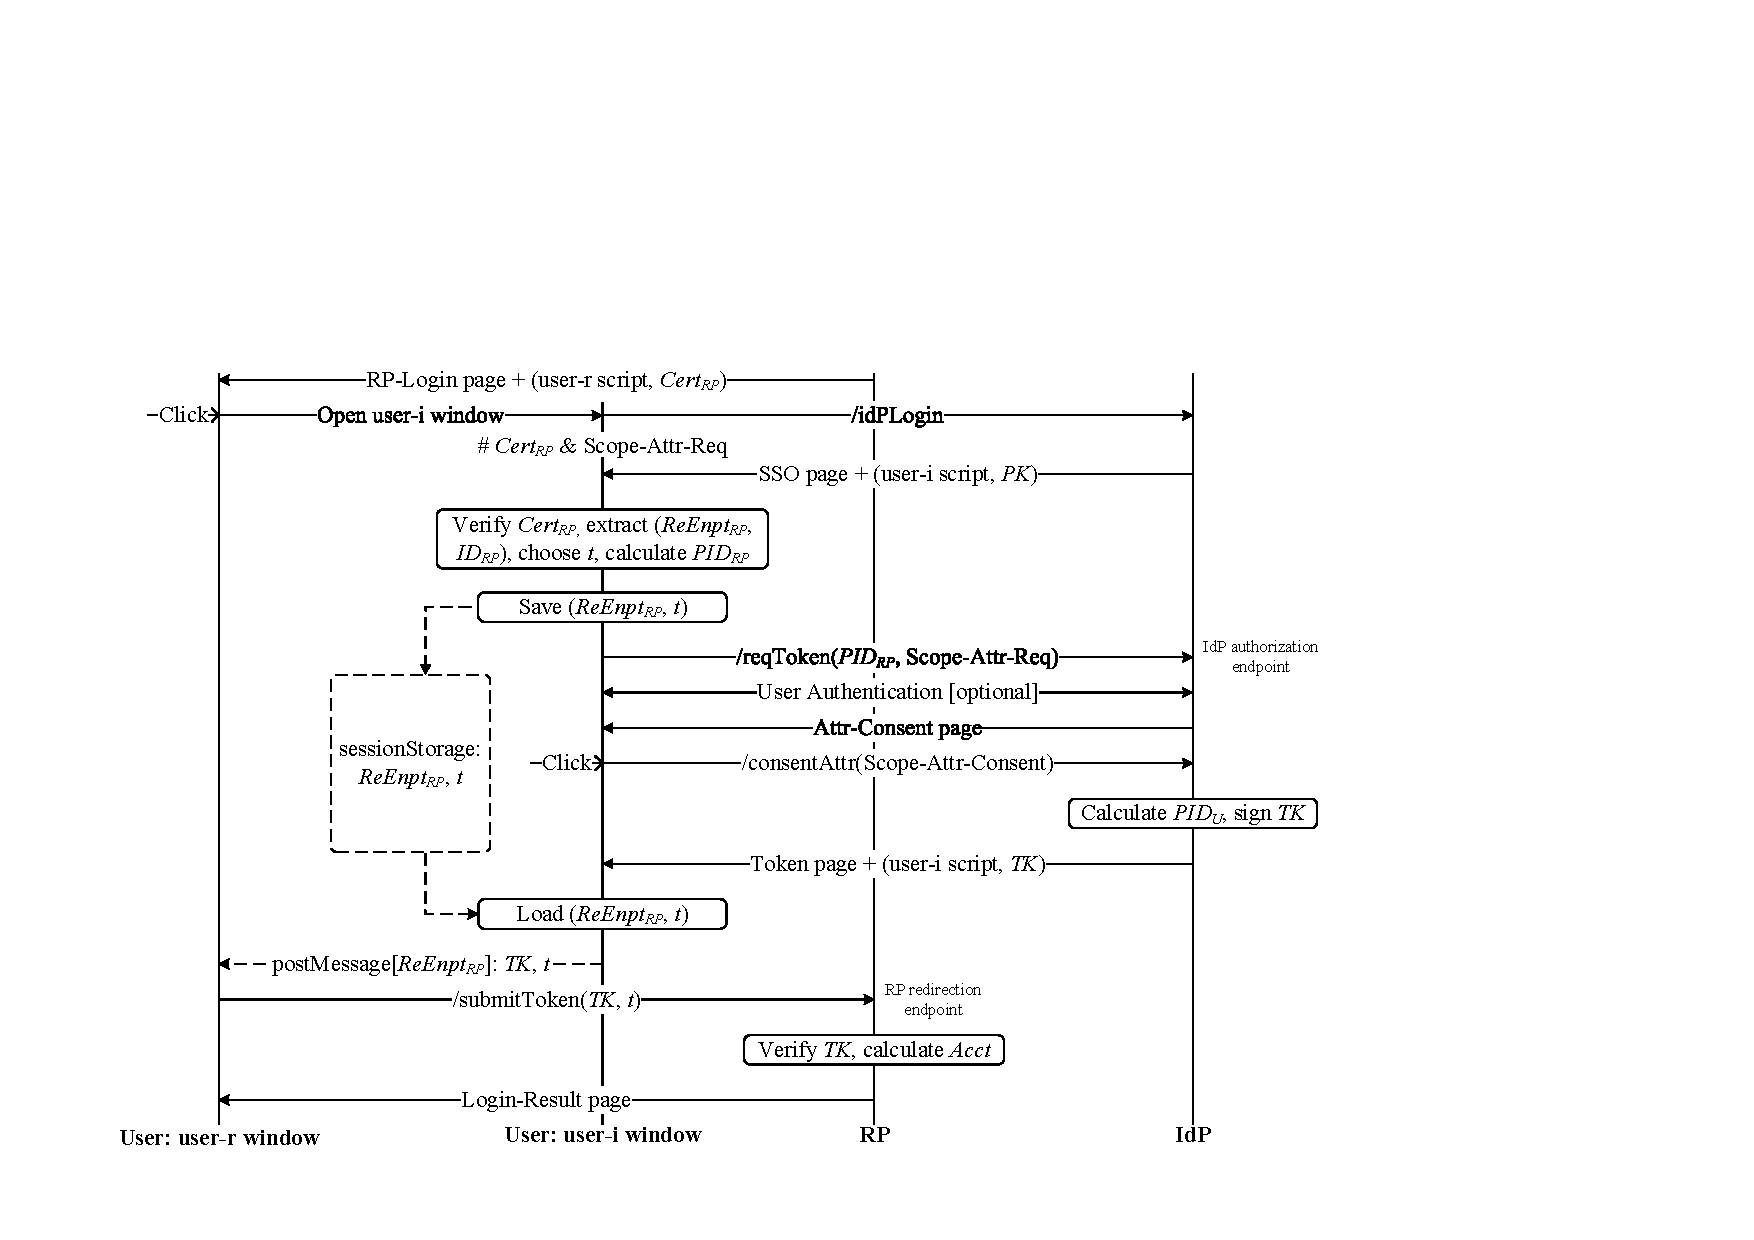
\includegraphics[width=0.785\linewidth]{fig/pop-up-process.pdf}
  \caption{The SSO login flow of UPPRESSO}
  \label{fig:process}
\end{figure*}



\subsection{The UPPRESSO protocol}
\label{implementations}

\noindent \textbf{System Initialization.}
$\mathbb{E}$, $G$ and $n$ are set up and publicly published.
An IdP generates a key pair ($SK$, $PK$) to sign and verify identity tokens and RP certificates.
%The IdP keeps $SK$ secret, and $PK$ is publicly known.


\noindent\textbf{RP Registration.}
Each RP registers itself at the IdP to obtain $ID_{RP}$ and its RP certificate $Cert_{RP}$ as follows.
This registration may be conducted by face-to-face means.
\begin{enumerate}
\setlength{\topsep}{0pt}
\setlength{\partopsep}{0pt}
\setlength{\itemsep}{0pt}
\setlength{\parsep}{0pt}
\setlength{\parskip}{0pt}
\item[1.]
An RP pre-installs $PK$ by trusted means.
It submits a registration request, including the endpoint to receive identity tokens and other information.
\item[2.]
After examining the request,
the IdP randomly selects $r \in \mathbb{Z}_n$
        and assigns a \emph{unique} point $[r]G$ to the RP as its identity.
Note that $r$ is not processed any more and then known to nobody
 due to the elliptic curve discrete logarithm problem (ECDLP).
%random number $r \in [1,n)$ until $ID_{RP} = [r]G$ is unique.
 %   but $r$ is kept unknown to the RP.
The IdP then signs $Cert_{RP} = [ID_{RP}, Enpt_{RP}, *]_{SK}$,
     where $[\cdot]_{SK}$ is a message signed using $SK$ and $*$ is supplementary information such as the RP's common name.
\item[3.]
The RP verifies $Cert_{RP}$ using $PK$, and accepts $ID_{RP}$ and $Cert_{RP}$.
\end{enumerate}


\noindent\textbf{User Registration.}
%Each user registers once at the IdP. 
Each user sets up her unique username and the corresponding credential for the IdP.
The IdP assigns
a unique random identity $ID_U = u\in \mathbb{Z}_n$ to the user.

It requires that $ID_U$ is known \emph{only} to the IdP.
In UPPRESSO $ID_U$ is used only by the IdP \emph{internally},
 not enclosed in any message.
%so a user inputs her username in the authentication to the IdP and $ID_U$ is processed only by the IdP internally.
For example, a user's identity is generated and always restored by hashing her username concatenated with the IdP's private key.
Then,
 $ID_U$ is never stored in hard disks,
 and protected almost the same as the IdP's private key
because it is \emph{only} used to calculate $PID_{U}$ as the IdP is signing an identity token binding $PID_{U}=
  [{ID_U}]{PID_{RP}}$.


\noindent\textbf{Account Synchronization.} 
% An account belonging to some registered user is \emph{meaningful}, while \emph{meaningless} accounts at an RP do not belong to any registered user.
Every RP regularly synchronizes all accounts at it from the IdP,
    and then locally maintains an up-to-date list of meaningful accounts.
We discuss account synchronization in Section \ref{account-syn}.


\noindent\textbf{SSO Login.} 
A login flow %is typically launched through a browser,
%when a user attempts to visit an RP. It
involves three steps: Identity-token requesting, generation, and acceptance.
In Figure \ref{fig:process}, the IdP's and RP's operations are connected by two vertical lines, respectively. The user operations are split into two groups in different browser windows by vertical lines, one communicating with the IdP and the other with the RP. Solid horizontal lines indicate messages exchanged between a user and the IdP (or the RP), while dotted lines represent the mechanisms within a browser:
(\emph{a}) \verb+postMessage+ invocations between two scripts (or browser windows)
or (\emph{b}) \verb+sessionStorage+ objects accessed by refreshed pages of an HTTP session.


\noindent 1. {\em Identity-Token Requesting.}
The user requests an identity token for $PID_{RP} = [t]{ID_{RP}}$.
\begin{itemize}
\setlength{\topsep}{0pt}
\setlength{\partopsep}{0pt}
\setlength{\itemsep}{0pt}
\setlength{\parsep}{0pt}
\setlength{\parskip}{0pt}
\item[1.1]
The target RP provides an SSO login page with the user-r script,
    and $Cert_{RP}$ is set in this script.
The user clicks the SSO login button,
    to pop up a new browser window responsible for communicating with the IdP.
\item[1.2] The user-i window downloads the user-i script,
which processes $Cert_{RP}$ and the scope of requested attributes sent from the user-r window.
It verifies $Cert_{RP}$, extracts $ID_{RP}$ and $Enpt_{RP}$ from $Cert_{RP}$, 
chooses a random number $t \in \mathbb{Z}_n$,
    and calculates $PID_{RP}=[t]{ID_{RP}}$.
\item[1.3] 
The user-i script uses the \verb+sessionStorage+ HTML5 object to save $Enpt_{RP}$ and $t$,
    and then requests an identity token from the IdP by sending $PID_{RP}$ and the scope of requested attributes.
\end{itemize}


\noindent 2. {\em Identity-Token Generation.}
The IdP calculates $PID_U = [ID_U]{PID_{RP}}$ and signs an identity token as follows. % The processes are as follows.
\begin{itemize}
\setlength{\topsep}{0pt}
\setlength{\partopsep}{0pt}
\setlength{\itemsep}{0pt}
\setlength{\parsep}{0pt}
\setlength{\parskip}{0pt}
\item[2.1]
On receiving an identity-token request,
the IdP authenticates the initiating user as $ID_U$, if not authenticated yet.
Then, it obtains the user's authorization to enclose attributes in the token.
\item[2.2]
The IdP calculates $PID_U = [ID_U]{PID_{RP}}$, and signs $TK = [PID_{RP}, PID_U, Iss, Validity, Attr]_{SK}$,
where $Iss$ identifies the IdP, $Validity$ indicates the validity period, and $Attr$ contains the authorized user attributes.
\item[2.3] The IdP replies with the identity token to the user-i window,
    as well as the user-i script to forward this token.
\end{itemize}


\noindent 3. {\em Identity-Token Acceptance.}
The RP receives the identity token and allows the user to log in.
\begin{itemize}
\setlength{\topsep}{0pt}
\setlength{\partopsep}{0pt}
\setlength{\itemsep}{0pt}
\setlength{\parsep}{0pt}
\setlength{\parskip}{0pt}
\item [3.1]
From the \verb+sessionStorage+ object
the user-i script loads $Enpt_{RP}$ and $t$, 
    and forwards the identity token and $t$ to the user-r window by \verb+postMessage+ which is restricted by $Enpt_{RP}$.
\item[3.2] Then, the user-r script submits it to the RP.
The RP verifies the signature and the validity period of the token, 
%Then, the RP extracts $PID_{RP}$ from the token, checks if it equals $[t]ID_{RP}$,
and calculates $Acct = [t^{-1}]{PID_U}$.

\item[3.3] Only if $Acct$ is meaningful in its local account list, the RP allows the user to log in.

\end{itemize}

If any verification fails, this login flow will be terminated immediately.
For example, the user halts it when receiving an invalid $Cert_{RP}$.
The IdP rejects an identity-token request if the received $PID_{RP}$ is not a point on $\mathbb{E}$, and the RP rejects the token holder if the identity token is invalid or the derived account is meaningless. 

In Step 3.2, an RP does not check whether $PID_{RP}$ enclosed in the signed token is equal to $[t]ID_{RP}$ or not,
    and this efficient design does not result in attacks, which is proved in Section \ref{analysis-security}.
It requires that in Step 3.3 the RP locally maintains an up-to-date account list,
    and account synchronization is explained with more details in Section \ref{account-syn}.

%%%%%%%%%%%%%%%%%%%%%%%%%%%%%%%%%%%%%%%%%%%%%%%%%%%%%%%%%%
% u泄露,则RP有必要比较!否则,就会伤害security。
%or the enclosed $PID_{RP}$ is not equal to $[t]ID_{RP}$.
%%%%%%%%%%%%%%%%%%%%%%%%%%%%%%%%%%%%%%%%%%%%%%%%%%%%%%%%%%
% 分析结论是:
% 现有的简化协议(RP不比较$PID_{RP}$是否相等),则:
% 当u不泄露,u的security和privacy都没有问题;
% 当u泄露,u的security和privacy都有问题。
%
% 改进协议(RP比较$PID_{RP}$是否相等),则:
% 当u不泄露,u的security和privacy都没有问题;
% 当u泄露,u的security没有问题,u的privacy有问题。
%%%%%%%%%%%%%%%%%%%%%%%%%%%%%%%%%%%%%%%%%%%%%%%%%%%%%%%%%%

%\subsection{Compatibility with OIDC}
%\label{subsec:compatible}
%
%\textbf{We do not mean IdP,
%but the OIDC protocol is used.}
%
%This threat model is in line with widely-used SSO services.
%
%An OIDC system works in two alternative modes \cite{dimvaLiM16,GoogleIdIntegrate,uber,de2014oauth}:
% pop-up UX with two web scripts, and redirect UX with only the user-r script.
%UPPRESSO only works in OIDC systems with pop-up UX. %(i.e., the communication flows among the IdP, the browser and the visited RP are identical),
%  %  while the downloaded scripts are modified to support identity transformations.
%%Both UPPRESSO and OIDC work with COTS browsers. %Among the four steps of the login flow
%%
%When a user attempts to visit an RP in UPPRESSO,
%        a user agent is prepared by two scripts in the \emph{script downloading} step.
%These scripts are downloaded, % following the same flow 
%like in OIDC systems with pop-up UX.
%%In UPPRESSO two scripts implement the verifications of RP certificates 
%%  and the user operations of identity transformations, in addition to attribute authorization and token receiving by the user-i script and token forwarding by the user-r script in original OIDC services.
%%
%%UPPRESSO employs web scripts to hide the RP's endpoint from the IdP, while securely forwarding identity tokens to the RP through $Enpt_{RP}$ extracted from the signed RP certificate.
%%Thus, the IdP cannot set \texttt{redirect_uri} in the HTTP responses, which is different from OIDC where HTTP redirections are used to implement these communications.
%%
%
%The \emph{RP identity transformation} step in UPPRESSO take place within a browser,
%            and the RP responds with its certificate after receiving $t$.
%The RP response is constructed following the standard format of OIDC requests \cite{dimvaLiM16},
%    but then processed by the user-i script to remove any information leaking the RP's identity.
%%which can be viewed as a supplementary access to static resources on the RP server.
%%The operations in the $PID_{RP}$ registration are almost identical to those in the RP Dynamic Registration of OIDC \cite{DynamicRegistration}, except that in OIDC the IdP assigns the RP's identity  while in UPPRESSO this (pseudo-)identity is generated by the registered entity. Besides, the $PID_{RP}$ registration has a validity period.
%
%The operations of \emph{identity-token generation} in UPPRESSO are compatible with those in OIDC,
% because (\emph{a}) the calculation of $PID_U$ is actually a special method to generate PPIDs and (\emph{b}) $PID_{RP}$ can be viewed as a ``dynamic'' RP pseudo-identity
%    so that \texttt{redirect\_uri} is missing in the responses by the IdP.
%%
%%Compared to the original OIDC protocol, UPPRESSO simplifies the IdP's operations in these two steps, while allowing ``dynamic'' RP pseudo-identities.
%Finally, the operations of \emph{$Acct$ calculation} in UPPRESSO are identical to those in OIDC,
% because the calculation of $Acct$ is a mapping from the user pseudo-identity enclosed in tokens to a local account at the visited RP.
%
%The compatibility is experimentally confirmed through our prototype implementation.
%When we built the IdP prototype of UPPRESSO on top of MITREid Connect \cite{MITREid},
%    only 23 lines of Java code are added:
%        three lines to calculate $PID_U$ as a special PPID using Java cryptographic libraries,
%    and 20 lines to support pop-up UX with identity transformations.
%%    modify the method of forwarding identity tokens.
